% questions.tex —— 1959 年·全国卷 · 题目内容片段（无答案）
% 由 tools/generate_projects.py 依来源总账自 1959/1959_数学真题_试题.md 生成，勿手改（改源 MD 后重跑）


\begin{gktip}
\textbf{题面说明}：原卷按“一（1）至（6）、二、三、四、五”编号，本文统一映射为第 1—10 题。题三原件印刷为面积 $\sqrt3$；纯文本提取会漏掉根号，本文按页面图像转录。
\end{gktip}

\gkpart{一、小题}

\begin{question}
\gkti{1}（1）已知 $\lg2=0.3010$，$\lg7=0.8451$，求 $\lg35$。

（注：$\lg$ 是以 $10$ 为底的对数的符号。）

\end{question}
\begin{question}
\gkti{2}（2）化简
\[
\frac{(1-\mathrm i)^3}{1+\mathrm i}.
\]

\end{question}
\begin{question}
\gkti{3}（3）解不等式：$2x^2+5x<3$。

\end{question}
\begin{question}
\gkti{4}（4）求 $\cos165^\circ$ 的值。

\end{question}
\begin{question}
\gkti{5}（5）一直圆台上底的面积为 $25\pi$ 平方厘米，下底的直径为 $20$ 厘米，母线长为 $10$ 厘米。求这直圆台的侧面积。

\Needspace{0.4\textheight}
\end{question}
\begin{question}
\gkti{6}（6）有三条不在同一平面内的平行线 $a$、$b$ 和 $c$。在线 $a$ 上取一固定线段 $AB$，在线 $c$、$b$ 上各任取一点 $C$ 和 $D$。求证：不论 $C$ 和 $D$ 取在 $c$、$b$ 的什么位置上，四面体 $ABCD$ 的体积总是不变的。
\nopagebreak[4]
\begin{center}% 1959 年全国卷第 6 题：三条互不共面的平行线与四面体 ABCD。
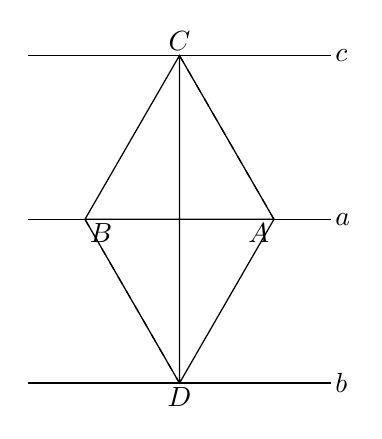
\begin{tikzpicture}[scale=0.8, line width=0.45pt,
  every node/.style={inner sep=1.5pt}]
  \coordinate (C) at (0,2.8); \coordinate (D) at (0,-2.4);
  \coordinate (B) at (-1.5,0.2); \coordinate (A) at (1.5,0.2);
  \draw (-2.4,2.8)--(2.4,2.8) node[anchor=west] {$c$};
  \draw (-2.4,0.2)--(2.4,0.2) node[anchor=west] {$a$};
  \draw (-2.4,-2.4)--(2.4,-2.4) node[anchor=west] {$b$};
  \draw (A)--(B)--(C)--cycle (A)--(D)--(B) (C)--(D);
  \draw[dashed] (C)--(A) (B)--(D);
  \draw[dashed] (C)--(D);
  \node[anchor=south] at (C) {$C$}; \node[anchor=north] at (D) {$D$};
  \node[anchor=north east] at (A) {$A$}; \node[anchor=north west] at (B) {$B$};
\end{tikzpicture}
\end{center}
\nopagebreak[4]
\end{question}
\gkpart{二、大题}

\begin{question}
\gkti{7}三个数成等差数列，前两个数的和的三倍等于第三个数的二倍；如果第二个数减去 $2$（仍当作第二项），三个数就成等比数列。求原来的三个数。

\end{question}
\begin{question}
\gkti{8}设有 $\triangle ABC$，已知 $\angle B=60^\circ$，$AC$ 边长为 $4$，面积为 $\sqrt3$。求 $AB$ 及 $BC$ 两边之长。

\end{question}
\begin{question}
\gkti{9}$A$、$B$、$C$ 是直线 $L$ 上三点，$P$ 是这直线外一点。已知 $AB=BC=a$，$\angle APB=90^\circ$，$\angle BPC=45^\circ$。试求：

（1）$\angle PBA$ 的正弦、余弦、正切；

（2）线段 $PB$ 的长；

（3）$P$ 点到直线 $L$ 的距离。

\Needspace{0.4\textheight}
\end{question}
\begin{question}
\gkti{10}延长圆 $O$ 的两弦 $AB$、$CD$ 交于圆外一点 $E$，过 $E$ 点作 $DA$ 的平行线交 $CB$ 的延长线于点 $F$，自 $F$ 点作圆 $O$ 的切线 $FG$。求证 $FG=FE$。
\nopagebreak[4]
\begin{center}% 1959 年全国卷第 10 题：圆外点 E、F 与两条割线和切线 FG。
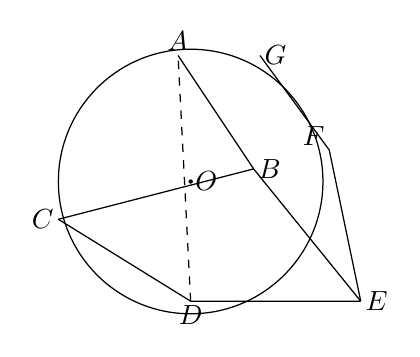
\begin{tikzpicture}[scale=0.8, line width=0.45pt,
  every node/.style={inner sep=1.5pt}]
  \coordinate (O) at (0,0); \coordinate (C) at (-2.1,-0.6); \coordinate (B) at (1.0,0.2);
  \coordinate (D) at (0.0,-1.9); \coordinate (A) at (-0.2,2.0);
  \coordinate (E) at (2.7,-1.9); \coordinate (F) at (2.2,0.5); \coordinate (G) at (1.1,2.0);
  \draw (O) circle (2.1);
  \draw (A)--(B)--(E) (C)--(D)--(E);
  \draw (E)--(F)--(G);
  \draw (C)--(B);
  \draw[dashed] (D)--(A);
  \fill (O) circle (0.035);
  \node[anchor=south] at (A) {$A$}; \node[anchor=west] at (B) {$B$};
  \node[anchor=east] at (C) {$C$}; \node[anchor=north] at (D) {$D$};
  \node[anchor=west] at (E) {$E$}; \node[anchor=south east] at (F) {$F$};
  \node[anchor=west] at (G) {$G$}; \node[anchor=west] at (O) {$O$};
\end{tikzpicture}
\end{center}
\nopagebreak[4]

\end{question}